\section{Kitting Problem}
\label{S:kitting-problem}
The kitting problem is quite complex and contains far too many states to represent them all explicitly. Using an example of kit to build, this section will only describe the initial and goal states explicitly. The operators detailed in Section~\ref{subsect:Planning_Operators} are used to generate the other states as needed. \\ \\
In this example, the \class{Robot} has to build a kit that contains two \class{Parts} of type A, one \class{Part} of type B and one \class{Part} of type C. The kitting process is completed once the kit is placed in the \class{LargeBoxWithKits}.
\paragraph{Constant Variable Symbols}
The kitting domain proposed for this example (Figure~\ref{fig:s0}) contains a \class{Robot} \const{r_1}, a \class{KitTray} \const{kt_1}, a \class{LargeBoxWithEmptyKitTrays} \const{lbwekt_1}, a \class{LargeBoxWithKits} \const{lbwk_1}, a \class{WorkTable} \const{wtable}, three \class{PartTrays} \const{pt_{A}}, \const{pt_{B}}, and \const{pt_{C}}, \class{Parts} \const{part_{A-1}}, \const{part_{A-2}}, \const{part_{B}}, and \const{part_{C}}, two \class{EndEffectors} \const{eff_1} and \const{eff_2}, and two  \class{EndEffectorHolders} \const{effh_1} and \const{effh_2}. Since a \class{KitInstance} is by definition a \class{KitTray} that contains \class{Parts}, the kitting domain also contains a constant variable symbol \const{kins_1} from \class{KitInstance}.


\subsection{State Variable Symbols}
The state variable symbols for the kitting domains are the ones defined in section \ref{subsubsect:State_Variable_Symbols}.

\subsection{Rigid Relations}

As stated in section \ref{subsubsect:Rigid_Relation}, the kitting domain has two rigid relations: \stvar{efftype} and \stvar{effhold-eff} that can be stated as follows:
\begin{itemize}
 \item \stvar{efftype}(\const{eff_1},\const{part_{A-1}})
 \item \stvar{efftype}(\const{eff_1},\const{part_{A-2}})
 \item \stvar{efftype}(\const{eff_1},\const{part_{B}})
 \item \stvar{efftype}(\const{eff_1},\const{part_{C}})
 \item \stvar{efftype}(\const{eff_2},\const{kt_1})
 \item \stvar{efftype}(\const{eff_2},\const{kins_1})
\end{itemize}


In the same way, \stvar{effhold-eff} can be stated as follows:
\begin{itemize}
 \item \stvar{effhold-eff}(\const{effh_1},\const{eff_1})
 \item \stvar{effhold-eff}(\const{effh_2},\const{eff_2})
\end{itemize}

\subsection{Initial State}
The initial state $s_0$ (Figure~\ref{fig:s0}) defines the predicates that are true in the kitting workstation. $s_0$ is represented in Table~\ref{table:initial}.

\begin{figure}[h!t!]
\centering
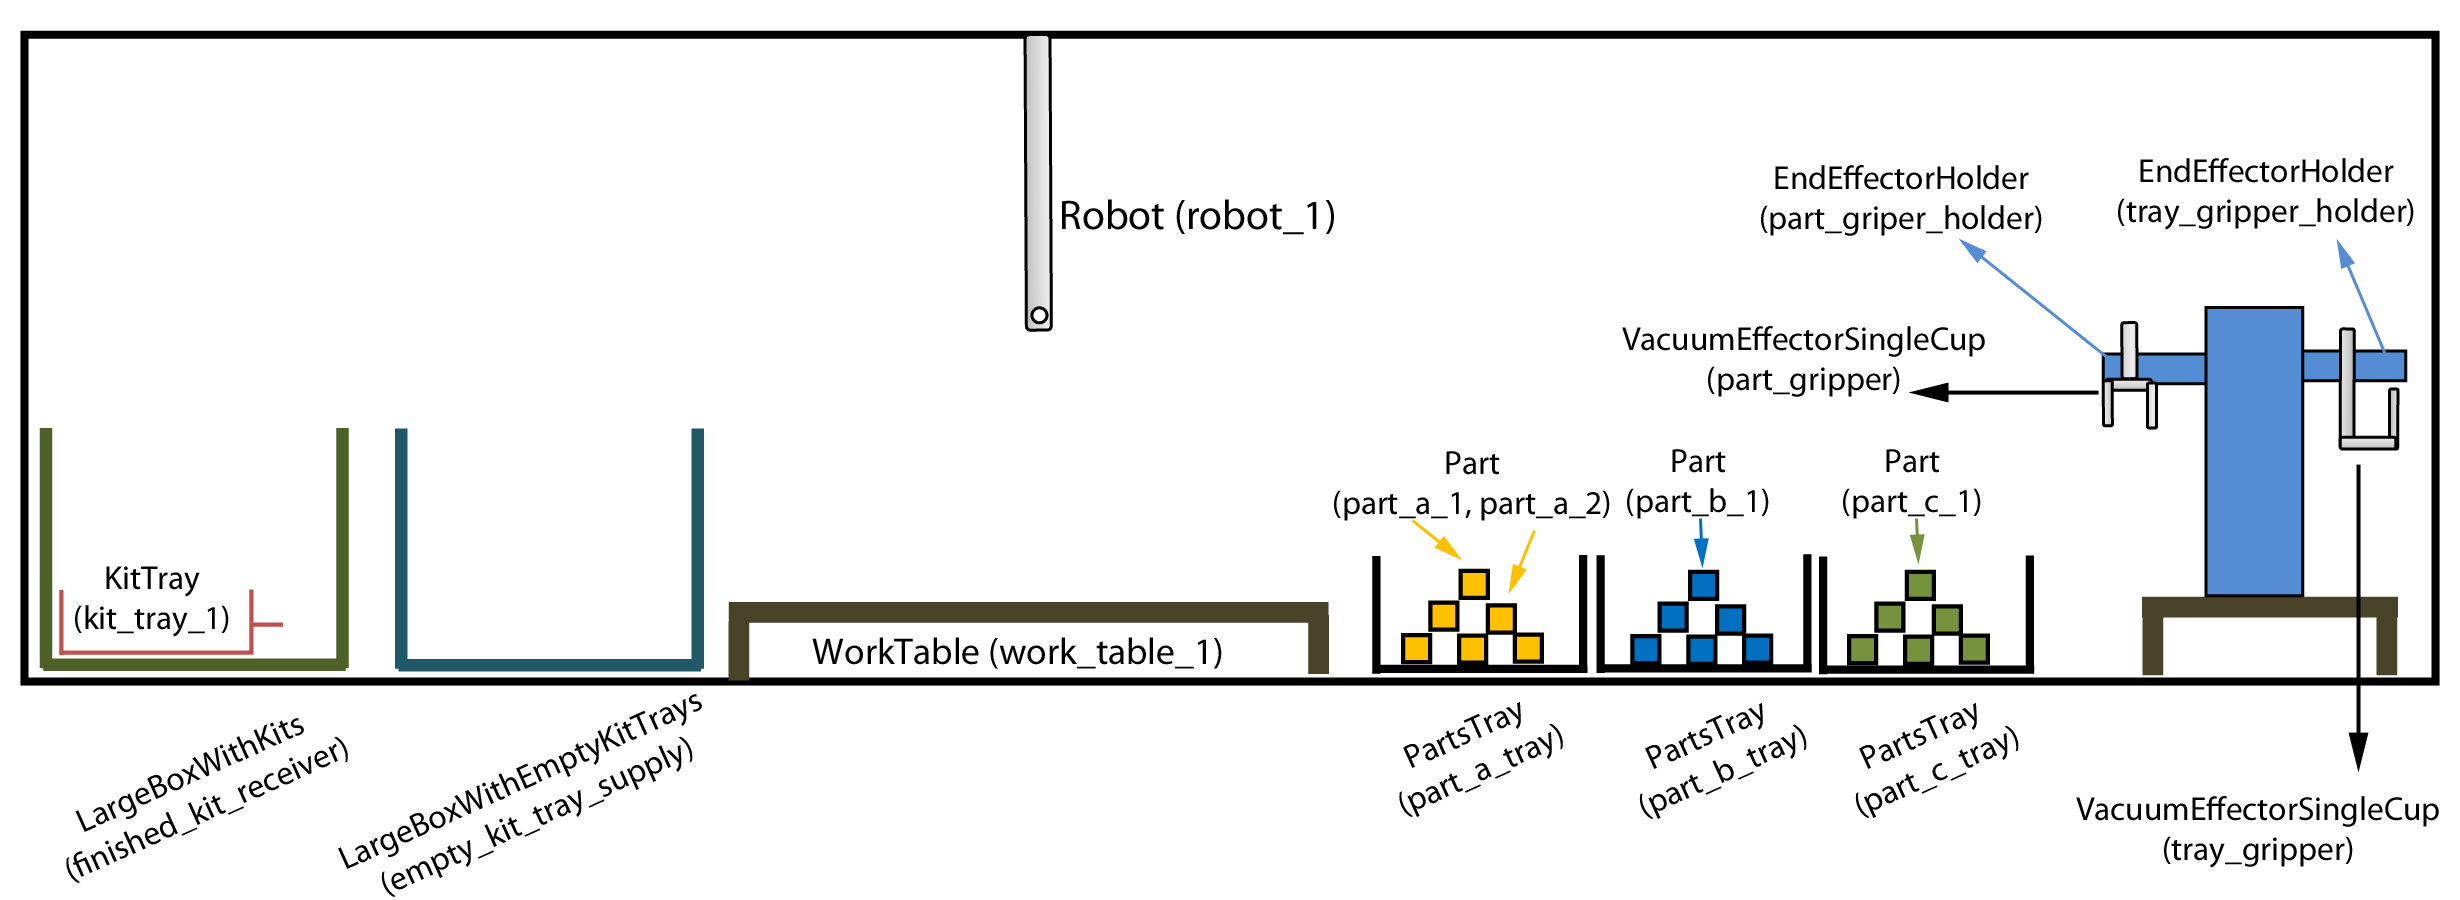
\includegraphics[width=16cm]{Figure/s0.jpg}
\caption{Initial state.}
\label{fig:s0}
\end{figure}


\begin{table}[h!t!p!]
\caption{Initial State $s_0$}
\centering
\begin{tabular}{|l|l|}
  \hline
  \hline
  \stvar{r-no-eff}(\const{r_1}) & \stvar{ktlocation}(\const{r_1},\const{lbwekt_1}) \\
  \stvar{lbwekt-non-empty}(\const{lbwekt_1}) & \stvar{partlocation}(\const{part_{A-1}},\const{pt_{A}}) \\
  \stvar{lbwek-non-full}(\const{lbwk_1}) & \stvar{partlocation}(\const{part_{A-2}},\const{pt_{A}}) \\
  \stvar{part-tray-non-empty}(\const{pt_{A}}) & \stvar{partlocation}(\const{part_{B}},\const{pt_{B}}) \\
  \stvar{part-tray-non-empty}(\const{pt_{B}}) & \stvar{partlocation}(\const{part_{C}},\const{pt_{C}}) \\
  \stvar{part-tray-non-empty}(\const{pt_{C}}) & \stvar{efftype}(\const{eff_1},\const{part_{A-1}}) \\
  \stvar{efflocation}(\const{eff_1},\const{effh_1}) & \stvar{efftype}(\const{eff_1},\const{part_{A-2}}) \\
  \stvar{efflocation}(\const{eff_2},\const{effh_2}) & \stvar{efftype}(\const{eff_1},\const{part_{B}}) \\
  \stvar{effhhold-eff}(\const{effh_1},\const{eff_1}) & \stvar{efftype}(\const{eff_1},\const{part_{C}}) \\
  \stvar{effhhold-eff}(\const{effh_2},\const{eff_2}) & \stvar{efftype}(\const{eff_2},\const{kt_1}) \\
  \stvar{worktable-empty}(\const{wtable}) & \stvar{efftype}(\const{eff_2},\const{kins_1})\\
  \hline
\end{tabular}
\label{table:initial}
\end{table}

\subsection{Goal State}

The goal state $s_G$ (Figure~\ref{fig:sf}) defines the predicates that are true in the final state. In the goal state, \class{Parts} \const{part_{A-1}}, \const{part_{A-2}}, \const{part_{B}}, and \const{part_{C}} are in the \class{KitInstance} \const{kins_1}. \const{kins_1} is placed in the \class{LargeBoxWithKits} \const{lbwk_1}. $s_G$ is represented in Table~\ref{table:final}.

\begin{table}[h!t!p!]
\caption{Final State $s_G$}
\centering
\begin{tabular}{|l|l|}
  \hline
  \hline
  \stvar{partlocation}(\const{part_{A-1}},\const{kins_1})\\
  \stvar{partlocation}(\const{part_{A-2}},\const{kins_1})\\
  \stvar{partlocation}(\const{part_{B}},\const{kins_1})\\
  \stvar{partlocation}(\const{part_{C}},\const{kins_1})\\
  \stvar{kinslocation}(\const{kins_1},\const{lbwk_1})\\
  \hline
\end{tabular}
\label{table:final}
\end{table}
\begin{figure}[h!t!]
\centering
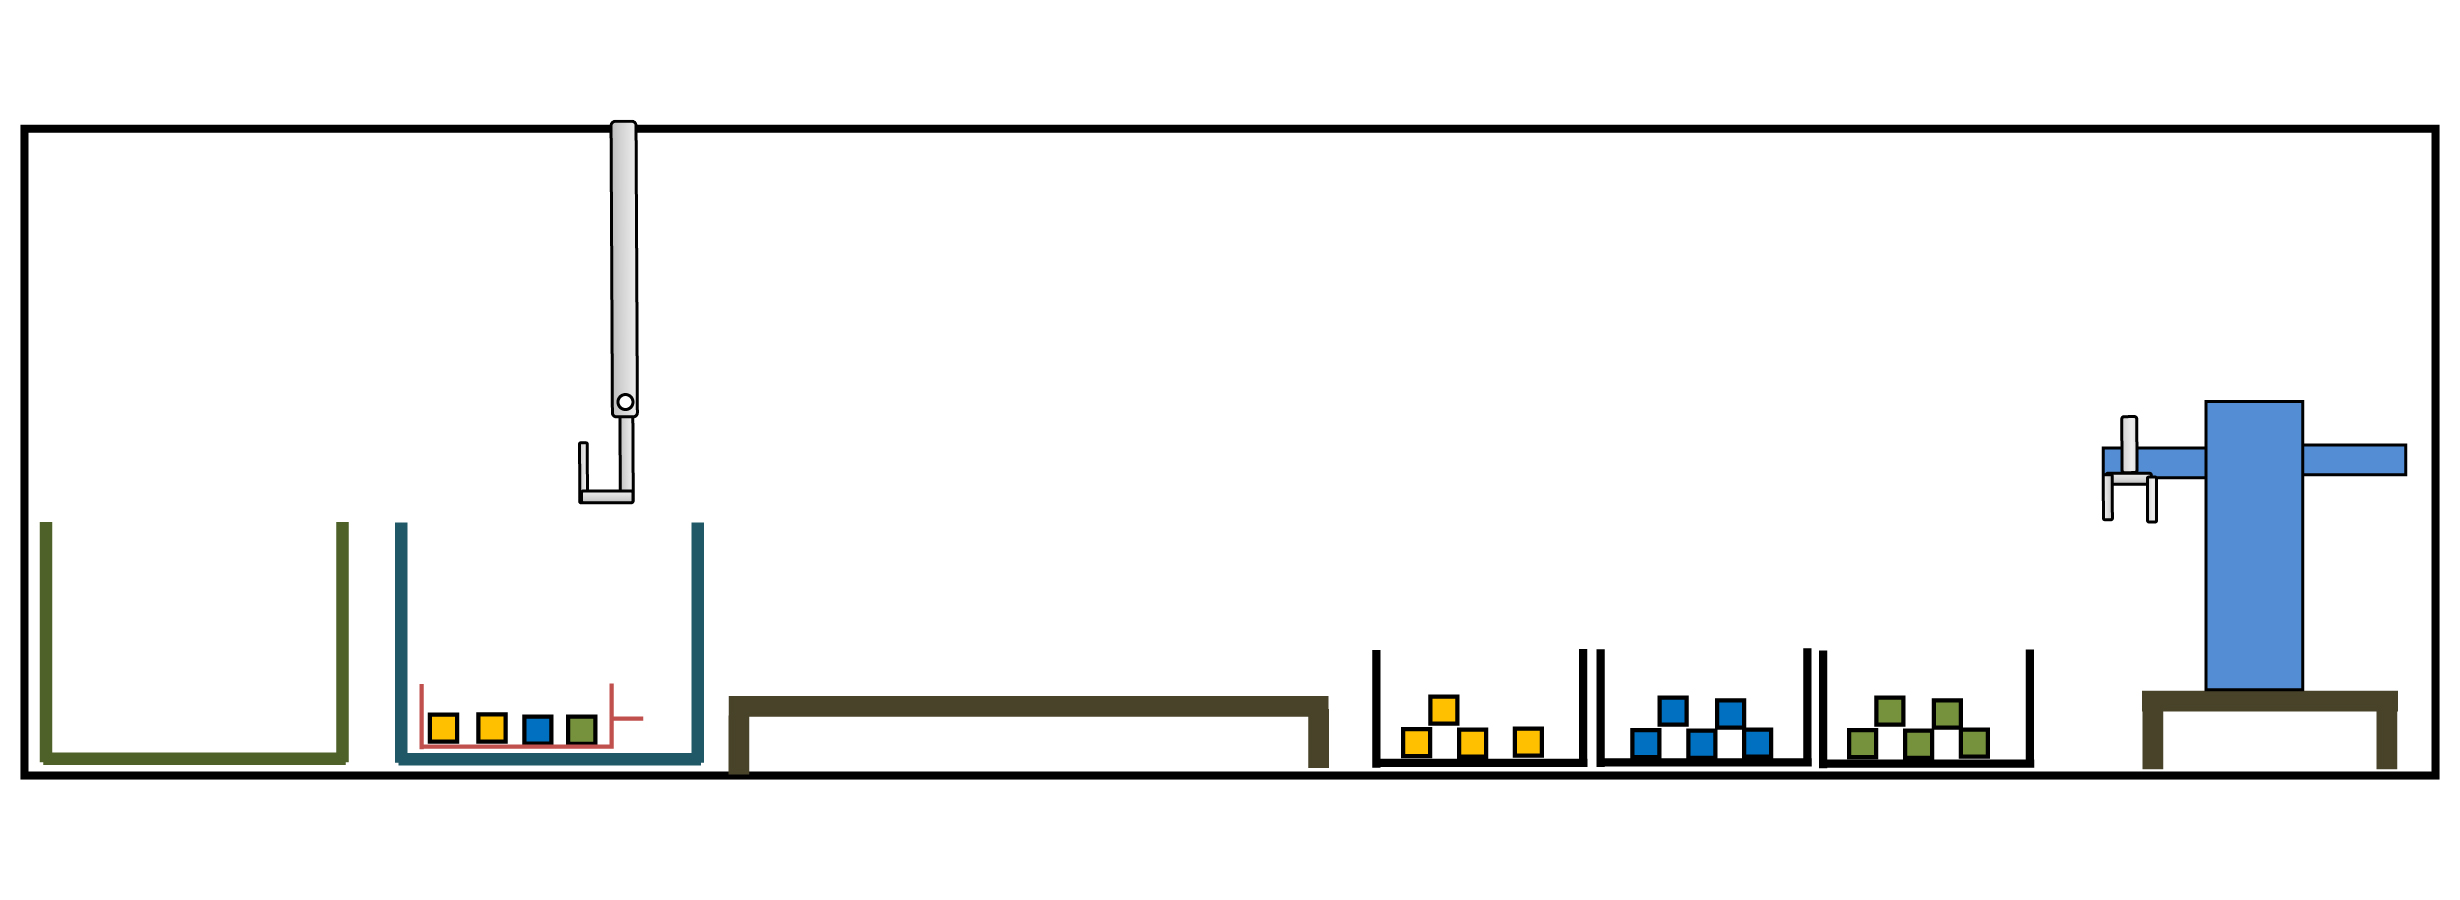
\includegraphics[width=16cm]{Figure/sfinal.jpg}
\caption{Goal state.}
\label{fig:sf}
\end{figure} 